%\AtBeginDvi{\special{pdf:mapfile texfonts.map}}
\documentclass[10pt]{jsarticle}
\usepackage{listings,jlisting}
\usepackage{color}
\usepackage{amsmath,amssymb}
\usepackage[dvipdfmx]{graphicx}
\usepackage{here}
\makeatletter
\def\lst@title@dropdelim\hskip1zw{}
\makeatother

%listingsの設定%{{{
\lstset{
    basicstyle = \small\ttfamily,    %ソースコードの書籍
    numbers = left,     %行番号
    numberstyle = \tiny,
    frame = {tblrTB},   %ソースコードを囲むフレーム(大文字があるところは二重線になる)
    backgroundcolor = {\color[gray]{.95}},  %数字を小さくすると黒くなる
    keywordstyle = {\small\bfseries \color[rgb]{0,0.4,0.4}},
    commentstyle = {\small\bfseries \color[rgb]{0.5,0.5,0.5}},
    identifierstyle={\small},%
    ndkeywordstyle={\small},%
    stringstyle={\small\ttfamily},
    columns=[l]{fullflexible},%
    keepspaces=true,
    showstringspaces=false,
    lineskip=-0.5zw,
}%}}}
\begin{document}
\begin{titlepage}
\title{情報実験第4 コンパイラ 課題2}
\date{\today}
\author{池田光 \\ 学籍番号:14\_00954 \\ ログイン名:j40095 \\メールアドレス:ikeda.h.am@m.titech.ac.jp}
\maketitle
\thispagestyle{empty}
\end{titlepage}

\section{目的}
以下をコンパイルできるように,コンパイラを拡張する.
\begin{enumerate}
  \item int型の局所変数
  \item int型の関数引数
  \item if文
  \item if-else文
  \item return
  \item ==式
  \item $\parallel$式
  \item \&\&式
  \item *式
  \item /式
\end{enumerate}
これらの実装により,int型の関数を含んだプログラムや,if文を含んだプログラム,四則演算を含んだプログラム(加算,減算は課題1にて実装済み),またはこれらを組み合わせたプログラムがコンパイル可能となる.

\section{変更点}
全ての変更はcodegen.hにて行った.

\subsection{visit\_AST関数について}
課題1の考察にもあげたが,右辺値と左辺値で取り扱い方が異なるため,1つのvisit\_ASTで扱うと分岐が煩雑になってしまうので,右辺値用にvisit\_AST\_right関数,左辺値用にvisit\_AST\_left関数を用意し,特別な扱いが必要な左辺値のみvisit\_AST\_left関数で扱い,その他をvisit\_AST\_rightで扱うことでこの問題の解決とした.また,この変更により,子から親の属性を見る必要がなくなるため実行速度の向上が期待される.
\subsection{共通の変更点}
\subsubsection{関数の宣言について}
課題1と同様,visit\_AST\_right関数内に代入式,if文,if-else文,return文,==式,$\parallel$式,*式,/のアセンブリコードを生成するための条件分岐及び関数を加えるとともに, プログラムの先頭に新たに追加した関数の定義をおこなう. これにより, 各ノードの属性に対応したアセンブリコードを出力する関数をvisit\_AST\_right関数内で呼び出しが可能となる.
以下に変更箇所を示す.
\begin{lstlisting}[caption=visit\_AST\_right関数]
  else if (!strcmp (ast->ast_type, "AST_expression_eq")){   // == 式
   codegen_expression_eq (ast);
 } else if (!strcmp (ast->ast_type, "AST_expression_lor")){  // ||式
   codegen_expression_lor (ast);
 } else if (!strcmp (ast->ast_type, "AST_expression_land")){  // &&式
   codegen_expression_land (ast);
 } else if (!strcmp (ast->ast_type, "AST_expression_mul")){  // *式
   codegen_expression_mul (ast);
 } else if (!strcmp (ast->ast_type, "AST_expression_div")){  // /式
   codegen_expression_div (ast);
 } else if (!strcmp (ast->ast_type, "AST_statement_if")){   //if文
   codegen_statement_if (ast);
 } else if (!strcmp (ast->ast_type, "AST_statement_ifelse")){ // ifelse文
   codegen_statement_ifelse (ast);
 } else if (!strcmp (ast->ast_type, "AST_statement_return")){ // return文
   codegen_statement_return (ast);
 }
\end{lstlisting}

\begin{lstlisting}[caption=関数の宣言]
  static void codegen_expression_eq(struct AST *ast);     //==式用関数の宣言
  static void codegen_expression_lor(struct AST *ast);     //||式用関数の宣言
  static void codegen_expression_land(struct AST *ast);    //&&式用関数の宣言
  static void codegen_expression_mul(struct AST *ast);    //*式用関数の宣言
  static void codegen_expression_div(struct AST *ast);    ///式用関数の宣言
  static void codegen_statement_if(struct AST *ast);     //if文
  static void codegen_statement_ifelse(struct AST *ast); //ifelse文
  static void codegen_statement_return(struct AST *ast); //return文
\end{lstlisting}

\subsubsection{スタックフレームについて}
課題1のときと同様に, 各関数内においてスタックから値を取り出したとき(pop を行ったとき)はframe\_heighから4を減算し,スタックへ値を積んだとき(pushを行うとき)はframe\_heightに4を加算する.この時,関数に入ったときと関数から出るときでframe\_heightを同じにしなければならない.詳細は後述する.

\subsection{int型の局所変数の実装}
codegen\_function\_definition関数にて定義を行う. AST.h内22行目にて,局所変数の合計サイズとして,total\_local\_sizeという変数が用意されているので,こちらを使用する.具体的には,total\_local\_sizeが0でない場合は領域の確保が必要となるため,この変数分\%espを減らすことで自動変数用の領域を確保するするアセンブリコードを出力するとともに,スタックフレームの高さをこの領域分増やすことで,局所変数の定義が完了する.\\
以下に局所変数の定義部分のコードを示す.
\begin{lstlisting}[caption=局所変数の定義]
  % if(ast->u.func.total_local_size != 0){
  %   emit_code (ast,"\tsubl\t$%d,%%esp\t#自動変数用\n",ast->u.func.total_local_size);
  %   frame_height += ast->u.func.total_local_size;
  % }
\end{lstlisting}

\par 局所変数はsymbol.h内15行目において,名前空間がNS\_Localであることがわかる.したがって,左辺値用と右辺値用のcodegen\_expression\_id\_left関数とcodegen\_expression\_id\_right関数のそれぞれにおいて名前空間のける分岐のNS\_Local部にて変更を加える. \\
\par codegen\_expression\_id\_rightについてはスタックに値をつむだけでよい.このとき,局所変数がベースポインタからどれくらい離れいるかをSymbol構造体のoffsetを用いて計算する.局所変数はint型なので,4バイトずつ積まれし,pushを行うアセンブリコードを出力する.\\
以下に変更点を示す.
\newpage
\begin{lstlisting}[caption=codegen\_expression\_id\_right関数内における局所変数]
  case NS_LOCAL:  //局所変数
    emit_code (ast,"\tpushl\t%d(%%ebp)\t\t#%sの内容をスタックに積む\n",symbol->offset*(-1)-4,id);
    frame_height += 4;
    break;
\end{lstlisting}

\par codegen\_expression\_id\_leftについては,左辺値なのでアドレスをスタックに積む必要がある.よって,leal命令によって使用する局所変数が格納されているアドレスを\%eaxに格納し,その後,\%eaxの値をスタックに積む.この時,codegen\_expression\_id\_right関数と同様にoffsetを用いて局所変数とベースポインターとの距離を計る.以上の過程のアセンブリコードを出力する.\\
以下に変更点を示す.
\begin{lstlisting}[caption=codegen\_expression\_id\_left関数内における局所変数]
  case NS_LOCAL:  //局所変数
    emit_code (ast,"\tleal\t%d(%%ebp),%%eax\t#左辺値\n",symbol->offset*(-1)-4);
    emit_code (ast,"\tpushl\t%%eax\n");
    frame_height += 4;
    break;
\end{lstlisting}


\subsection{int型の関数引数の実装}
関数呼び出し時において,16バイト境界条件を満たすようにpaddingを計算し積む必要があるが,これはcodegen\_expression\_funcall関数内にて実装されている.この関数では必要なpaddingを積んだのち,子ノード に対しvisit\_AST\_right関数を呼ぶことで引数の値を積み関数を呼び出している.最後に引数とpaddingを捨て関数を終わる.したがって,子ノードに対してvisit\_AST\_right関数が呼ばれ,関数引数に対する属性はAST\_expression\_idなのでcodegen\_expression\_id\_right関数とcodegen\_expression\_id\_left関数内にて変更を行う.さらに,関数引数はsymbol.h内16行目において,名前空間がNS\_ARGであることがわかる.したがって,codegen\_expression\_id\_right関数とcodegen\_expression\_id\_left関数のそれぞれにおいて名前空間における分岐のNS\_ARG部にて変更を行う.
\par 2つともおおよその変更は局所変数の際と同じであるが,関数引数はint型であるので,ベースポインターから戻り番地を挟んで4バイトずつ足された方向に増えるので関数引数とベースポインタとの距離を計算する部分のみ局所変数と異なる.\\
以下に変更点を示す.
\begin{lstlisting}[caption=codegen\_expression\_id\_right関数内における関数引数]
  case NS_ARG:    //引数
    emit_code (ast,"\tpushl\t%d(%%ebp)\t\t#%sの内容をスタックに積む\n",symbol->offset+8,id);
    frame_height += 4;
    break;
\end{lstlisting}

\begin{lstlisting}[caption=codegen\_expression\_id\_left関数内における関数引数]
  case NS_ARG:    //引数
    emit_code (ast, "\tleal \t%d(%%ebp), %%eax\t#左辺値\n",symbol->offset + 8);
    emit_code (ast, "\tpushl \t%%eax\n");
    frame_height += 4;
    break;
\end{lstlisting}


\subsection{if文について}
if文のアセンブリコードの生成はcodegen\_statement\_if関数にて行う.
\par はじめに,0番目の子ノードについてvisit\_AST\_right関数を呼び出すことで,条件式のアセンブリコードを出力する.条件式の計算結果と0を比べることで,条件式の真偽を判定する.次に,条件式が偽であった場合のジャンプ命令を出力し,ジャンプしなかった(条件式が真であった)場合のif文内の処理(1番目の子ノード)をvisit\_AST\_right関数を呼ぶことでアセンブリコードを出力する.最後に,条件式が偽であった場合のジャンプ先のラベルを出力する.以上により,if文のアセンブリコードを出力することが出来,if文を含むプログラムのコンパイルが可能となる.
\par ラベルに関しては,if文の中と外を分ける必要があり,既存のラベル以外に一つ必要であり,if文内でlabel\_ifに現在のlabelを代入し,labelをインクリメントすることで条件を満たす. \\
以下に変更点を示す.
\begin{lstlisting}[caption=codegen\_statement\_if関数]
  % static void
  % codegen_statement_if (struct AST *ast)
  % {
  %   visit_AST_right(ast->child[0]);
  %   emit_code(ast, "\tpopl\t%%eax\n");
  %   frame_height -= 4;
  %   emit_code(ast, "\tcmpl\t$0,%%eax\n");
  %   int label_if = label;
  %   label += 1;
  %   emit_code(ast,"\tje\tL%d\n",label_if);
  %   visit_AST_right(ast->child[1]);
  %   emit_code(ast,"L%d:\n",label_if);
  % }
\end{lstlisting}

\subsection{if-else文について}
if-else文のアセンブリコードの生成はcodegen\_statement\_ifelse関数で行う.
\par はじめに,0番目の子ノードについてvisit\_AST\_right関数を呼び出すことで,条件式のアセンブリコードを出力する.条件式の計算結果と0を比べることで,条件式の真偽を判定し,条件式が偽であった場合のラベルへのジャンプ命令を出力する.子ノードの1番目についてvisit\_AST\_right関数を呼び出すことでif文の中の処理に対するアセンブリコードを出力する.次に,if-else文の出口への無条件ジャンプ命令を出力する.条件式が偽であった場合のラベルを出力し,2番目の子ノードについてvisit\_AST\_right関数を呼び出すことでelse文内の処理に対するアセンブリコードを出力する.最後にif-else文のを出た時のラベルに対するアセンブリコードを出力する.以上により,if-else文のアセンブリコードを出力することが出来,if-else文を含むプログラムのコンパイルが可能となる.
\par ラベルに関しては,if文内・else文内・if-elseの出口の3つ必要だが,既存のラベル以外に2つ必要であり,if-else文内でlabel\_ifelseに現在のlabelを代入し,labelに2を加えることで条件を満たす.\\
以下に変更点を示す.
\begin{lstlisting}[caption=codegen\_statement\_ifelse]
  % static void
  % codegen_statement_ifelse (struct AST *ast)
  % {
  %    visit_AST_right(ast->child[0]);
  %    emit_code(ast,"\tpopl\t%%eax\n");
  %    frame_height -= 4;
  %    emit_code(ast,"\tcmpl\t$0,%%eax\n");
  %    int label_ifelse = label;
  %    label += 2;
  %    emit_code(ast,"\tje\tL%d\n",label_ifelse);
  %    visit_AST_right(ast->child[1]);
  %    emit_code(ast,"\tjmp\tL%d\n",label_ifelse+1);
  %    emit_code(ast,"L%d:\t\t\t\t\t#elseのとき\n",label_ifelse);
  %    visit_AST_right(ast->child[2]);
  %    emit_code(ast,"L%d:\t\t\t\t\t#ifelseの出口\n",label_ifelse+1);
  % }
\end{lstlisting}

\subsection{return文について}
return文のアセンブリコード生成はcodegen\_statement\_return関数にて行う.
\par return文では返り値を伴うものと伴わないものがあるので,0番目の子ノードの属性によって場合分けをする.属性がAST\_expression\_opt\_singleのとき,返り値を伴うので,visit\_AST\_right関数にて子ノードのアセンブリコードを出力し,\%eaxをpopする.\\
最後に,関数から抜け出すための無条件ジャンプ命令を出力する. 以上により,return文に対するアセンブリコードの生成が可能となる.\\
以下に変更点を示す.
\begin{lstlisting}[caption=codegen\_statement\_return関数]
  static void
  codegen_statement_return (struct AST *ast)
  {
    if(!strcmp(ast->child[0]->ast_type,"AST_expression_opt_single")){
      visit_AST_right(ast->child[0]);
      emit_code(ast,"\tpopl\t%%eax\n");
      frame_height -= 4;
    }
    emit_code(ast,"\tjmp\tL.XCC.RE.%s\t#return\n",funcname);
  }
\end{lstlisting}


\subsection{==式について}
==式のアセンブリコードの生成はcodegen\_expression\_eq関数で行う.
\par  はじめに,子ノードを左辺式,右辺式と順にvisit\_AST\_right関数にて処理し,スタックから順にpopし\%ecx,\%eaxに順に格納する.次に\%ecxと\%eaxをcmpl命令により比較し,seteを用いて比較結果を\%alに保存する.sete命令は直前の比較演算結果が同じ場合\%alを1に,そうでない場合0にする.その後,\%alの値を\%eaxにmovzbl命令を用いてコピーをし,スタックに積む.このmovzbl命令は8bitレジスタ\%alの値を32bitレジスタ\%eaxにコピーする命令である.最後に\%eaxの値をスタックに積む.以上のアセンブリコードを出力することで,if文の条件などで==式を利用したプログラムがコンパイル可能となる.\\
以下に変更点を示す.
\begin{lstlisting}[caption=codegen\_expression\_eq関数]
  static void
  codegen_expression_eq (struct AST *ast)
  {
    int i;
    for (i=0; i < ast->num_child; i++){
      visit_AST_right(ast->child[i]);
    }
    emit_code(ast,"\tpopl\t%%ecx\n");
    frame_height -= 4;
    emit_code(ast,"\tpopl\t%%eax\n");
    frame_height -= 4;
    emit_code(ast,"\tcmpl\t%%ecx,%%eax\n");
    emit_code(ast,"\tsete\t%%al\t\t# ==式\n");
    emit_code(ast,"\tmovzbl\t%%al,%%eax\n");
    emit_code(ast,"\tpushl\t%%eax\n");
    frame_height += 4;
  }
\end{lstlisting}

\subsection{$\parallel$式について}
$\parallel$式のアセンブリコードの生成はcodegen\_expression\_lor関数で行う.
\par はじめに,0番目の子ノードをvisit\_AST\_right関数にてアセンブリコードを出力するとともに左辺値をスタックに積む.この値と0とをcmpl命令にて比較し,真偽判定を行う.真であった場合,右辺値にかかわらず条件式は真になるので,ジャンプ命令を行いスタックに1を積む.偽の場合,1番目の子ノードをvisit\_AST\_right関数にてアセンブリコードを出力するとともに右辺値のをスタックに積む.この値と0とをcmple命令にて比較し,真偽を判定する.真であった場合,左辺値が真であったときと同じラベルにジャンプし,1をスタックに積む.偽の場合,左辺値も右辺値も偽となるので,新しいラベルにジャンプし,0をスタックに積む.
\par 以上のアセンブリコードを出力することで,or演算を含むプログラムのコンパイルが可能となる.\\
\par $\parallel$式においてlabelを2つ使っているので,labelに2を加える.また,関数を呼び出したときと終了時ではスタックフレームの高さが同じではないといけないこと,静的にみるとpushを2回おこなっているので,frame\_hightを8加える必要があるように見えるが,実際はいずれかのpushが行われるのでframe\_heightは4を加えるだけでよい.
以下に変更点を示す.
\begin{lstlisting}[caption=codegen\_expression\_lor関数]
  static void
  codegen_expression_lor (struct AST *ast)
  {
    int label_lor = label;
    label += 2;
    visit_AST_right(ast->child[0]);
    emit_code(ast,"\tpopl\t%%eax\n");
    frame_height -= 4;
    emit_code(ast,"\tcmpl\t$0,%%eax\n");
    emit_code(ast,"\tjne\tL%d\n",label_lor);
    visit_AST_right(ast->child[1]);
    emit_code(ast,"\tpopl\t%%eax\n");
    frame_height -= 4;
    emit_code(ast, "\tcmpl \t$0, %%eax\n");
    emit_code(ast, "\tjne \tL%d\n",label_lor);
    emit_code(ast, "\tpushl \t$0\n");
    // frame_height +=4;
    emit_code(ast, "\tjmp \tL%d\n",label_lor + 1);
    emit_code(ast, "L%d:\t\t\t\t\t# || in\n",label_lor);
    emit_code(ast, "\tpushl \t$1\n");
    frame_height += 4;
    emit_code(ast, "L%d:\t\t\t\t\t# || out\n",label_lor + 1);
  }
\end{lstlisting}

\subsection{\&\&式について}
\&\&式のアセンブリコードの生成はcodegen\_expression\_land関数で行う.
\par はじめに,0番目の子ノードをvisit\_AST\_right関数にてアセンブリコードを出力するとともに左辺値をスタックに積む.この値と0とをcmpl命令にて比較し,真偽判定を行う.偽であった場合,右辺値にかかわらず条件式は偽になるので,ジャンプ命令を行いスタックに0を積む.真の場合,1番目の子ノードをvisit\_AST\_right関数にてアセンブリコードを出力するとともに右辺値のをスタックに積む.この値と0とをcmple命令にて比較し,真偽を判定する.偽であった場合,左辺値が偽であったときと同じラベルにジャンプし,0をスタックに積む.真の場合,左辺値も右辺値も真となるので,新しいラベルにジャンプし,1をスタックに積む.
\par 以上のアセンブリコードを出力することで,and演算を含むプログラムのコンパイルが可能となる.\\
\par \&\&式においてlabelを2つ使っているので,labelに2を加える.また,関数を呼び出したときと終了時ではスタックフレームの高さが同じではないといけないこと,静的にみるとpushを2回おこなっているので,frame\_hightを8加える必要があるように見えるが,実際はいずれかのpushが行われるのでframe\_heightは4を加えるだけでよい.
以下に変更点を示す.
\begin{lstlisting}[caption=codegen\_expression\_land]
  static void
  codegen_expression_land (struct AST *ast)
  {
    int label_land = label;
    label += 2;   //条件内と外の2つ
    visit_AST_right(ast->child[0]);
    emit_code(ast,"\tpopl\t%%eax\n");
    frame_height -= 4;
    emit_code(ast,"\tcmpl\t$1,%%eax\n");
    emit_code(ast,"\tjne\tL%d\n",label_land);
    visit_AST_right(ast->child[1]);
    emit_code(ast,"\tpopl\t%%eax\n");
    frame_height -= 4;
    emit_code(ast,"\tcmpl\t$1,%%eax\n");
    emit_code(ast,"\tjne\tL%d\n",label_land);
    emit_code(ast,"\tpushl\t$1\n");
    // frame_height += 4;
    emit_code(ast,"\tjmp\tL%d\n",label_land+1);
    emit_code(ast,"L%d:\t\t\t\t\t# && in\n",label_land);
    emit_code(ast,"\tpushl\t$0\n");
    frame_height += 4;
    emit_code(ast,"L%d:\t\t\t\t\t# && out\n",label_land+1);
  }
\end{lstlisting}

\subsection{*式について}
*式のアセンブリコードの生成はcodegen\_expression\_mul関数にて行う.
\par はじめに, 左辺式と右辺式を順にvisit\_AST\_right関数にて処理をし, それぞれの値をスタックに積んだ後, スタックから順にpopし\%ecx,\%eaxに格納する. 次に,imull命令を用いて\%ecxと\%eaxの掛け算を行い,結果が格納された\%eaxをスタックに積む.
\par 以上のアセンブリコードを出力することで, 掛け算についてコンパイルすることが可能となった. \\
以下にコードを示す.
\begin{lstlisting}[caption=codegen\_expression\_mul]
  static void
  codegen_expression_mul(struct AST *ast)
  {
    int i;
    for(i=0; i < ast->num_child; i++){
      visit_AST_right(ast->child[i]);
    }
    emit_code(ast,"\tpopl\t%%ecx\n");
    frame_height -= 4;
    emit_code(ast,"\tpopl\t%%eax\n");
    frame_height -= 4;
    emit_code(ast,"\timull\t%%ecx,%%eax\t# 掛け算\n");
    emit_code(ast,"\tpushl\t%%eax\n");
    frame_height += 4;
  }
\end{lstlisting}

\subsection{/式について}
/式のアセンブリコードの生成はcodegen\_expression\_div関数にて行う.
\par はじめに, 左辺式と右辺式を順にvisit\_AST\_right関数にて処理をし, それぞれの値をスタックに積んだ後, スタックから順にpopし\%ecx,\%eaxに格納する. 次に,cltd命令により符号拡張した後,idivl令を用いて\%ecxと\%eaxの掛け算を行い,結果が格納された\%eaxをスタックに積む.
\par 以上のアセンブリコードを出力することで, 割り算についてコンパイルすることが可能となった. \\
以下にコードを示す.
\begin{lstlisting}[caption=codegen\_expression\_div]
  static void
  codegen_expression_div (struct AST *ast)
  {
    int i;
    for(i=0; i < ast->num_child; i++){
      visit_AST_right(ast->child[i]);
    }
    emit_code(ast,"\tpopl\t%%ecx\n");
    frame_height -= 4;
    emit_code(ast,"\tpopl\t%%eax\n");
    frame_height -= 4;
    emit_code(ast,"\tcltd\n");
    emit_code(ast,"\tidivl\t%%ecx,%%eax\t# 割り算\n");
    emit_code(ast,"\tpushl\t%%eax\n");
    frame_height += 4;
  }
\end{lstlisting}

\section{例プログラムと実行結果}

\subsection{例プログラムと自作プログラム}

\lstinputlisting[caption=例プログラム]{kadai2.c}
\lstinputlisting[caption=自作プログラム]{kadai2-2.c}

\subsection{例プログラムの実行結果}
\begin{figure}[htbp]
 \begin{minipage}{0.5\hsize}
  \begin{center}
   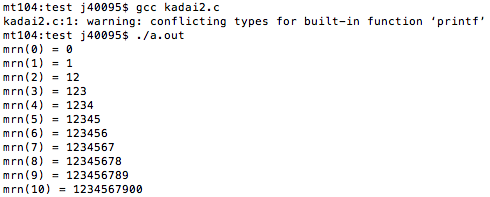
\includegraphics[width=70mm]{kadai2-gcc.png}
  \end{center}
  \caption{gccでの実行結果}
 \end{minipage}
 \begin{minipage}{0.5\hsize}
  \begin{center}
   \includegraphics[width=70mm]{kadai2-xcc.png}
  \end{center}
  \caption{xccでの実行結果}
 \end{minipage}
\end{figure}

\newpage

\subsection{自作プログラムの実行結果}
\begin{figure}[htbp]
 \begin{minipage}{0.5\hsize}
  \begin{center}
   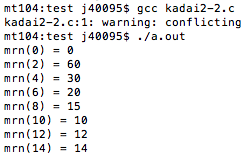
\includegraphics[width=70mm]{kadai2-2-gcc.png}
  \end{center}
  \caption{gccでの実行結果}
 \end{minipage}
 \begin{minipage}{0.5\hsize}
  \begin{center}
   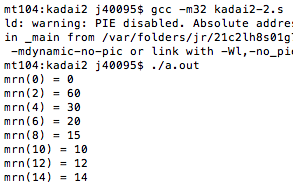
\includegraphics[width=70mm]{kadai2-2-xcc.png}
  \end{center}
  \caption{xccでの実行結果}
 \end{minipage}
\end{figure}

\section{評価}
すべての課題を実装し,実行結果も正しいものとなったが,MieruCompilerに頼ってしまった部分が多かったのが残念であった.

\section{考察}
or演算子とand演算子において,実際の動きを考えずpushが2回されたので2回frame\_heightを増やしてしまい,余計なpaddingを積んでしまっていた.
前回の課題と今回の課題において,pushやpopを行った際,frame\_heightをその都度変えていたが,必要なときはその都度変更をし,
その他の場合は,関数の最後にまとめて行うことで,上記のエラーは起こらなくなると考えた.

\section{まとめ}
今回の課題で,局所変数や関数引数の処理を行ったことで,スタックフレームの使われ方や構造をより深く理解することが出来た.
原理と実際の挙動を考えてしっかりコードを書くことを忘れずに行っていく必要があると改めて強く感じた.

\end{document}
